\documentclass[12pt]{article}
\usepackage{graphicx}
\usepackage{amsmath}
\usepackage{geometry}
\geometry{margin=1in}

\title{ECE 60141: Foundations of Computational Imaging\\Lab 3: Linear Forward Models and MAP Reconstruction}
\author{William Yau}
\date{2026/09/20}

\begin{document}

\maketitle

\section*{D1: Forward and Adjoint Operator Analysis}

\subsection*{Kernel Properties}

The blur kernel $\mathbf{a}$ was loaded from \texttt{levin09\_kernel1.txt} with the following properties:
\begin{itemize}
    \item Shape: $19 \times 19$
    \item Sum: $\sum \mathbf{a} = 1.0$ (normalized)
\end{itemize}

\subsection*{Results}

The figure below shows the comparison between the forward operator $A\mathbf{x}$ and the adjoint operator $A^T\mathbf{x}$ applied to the image $\mathbf{x}$ (kodim23.pgm):

\begin{center}
    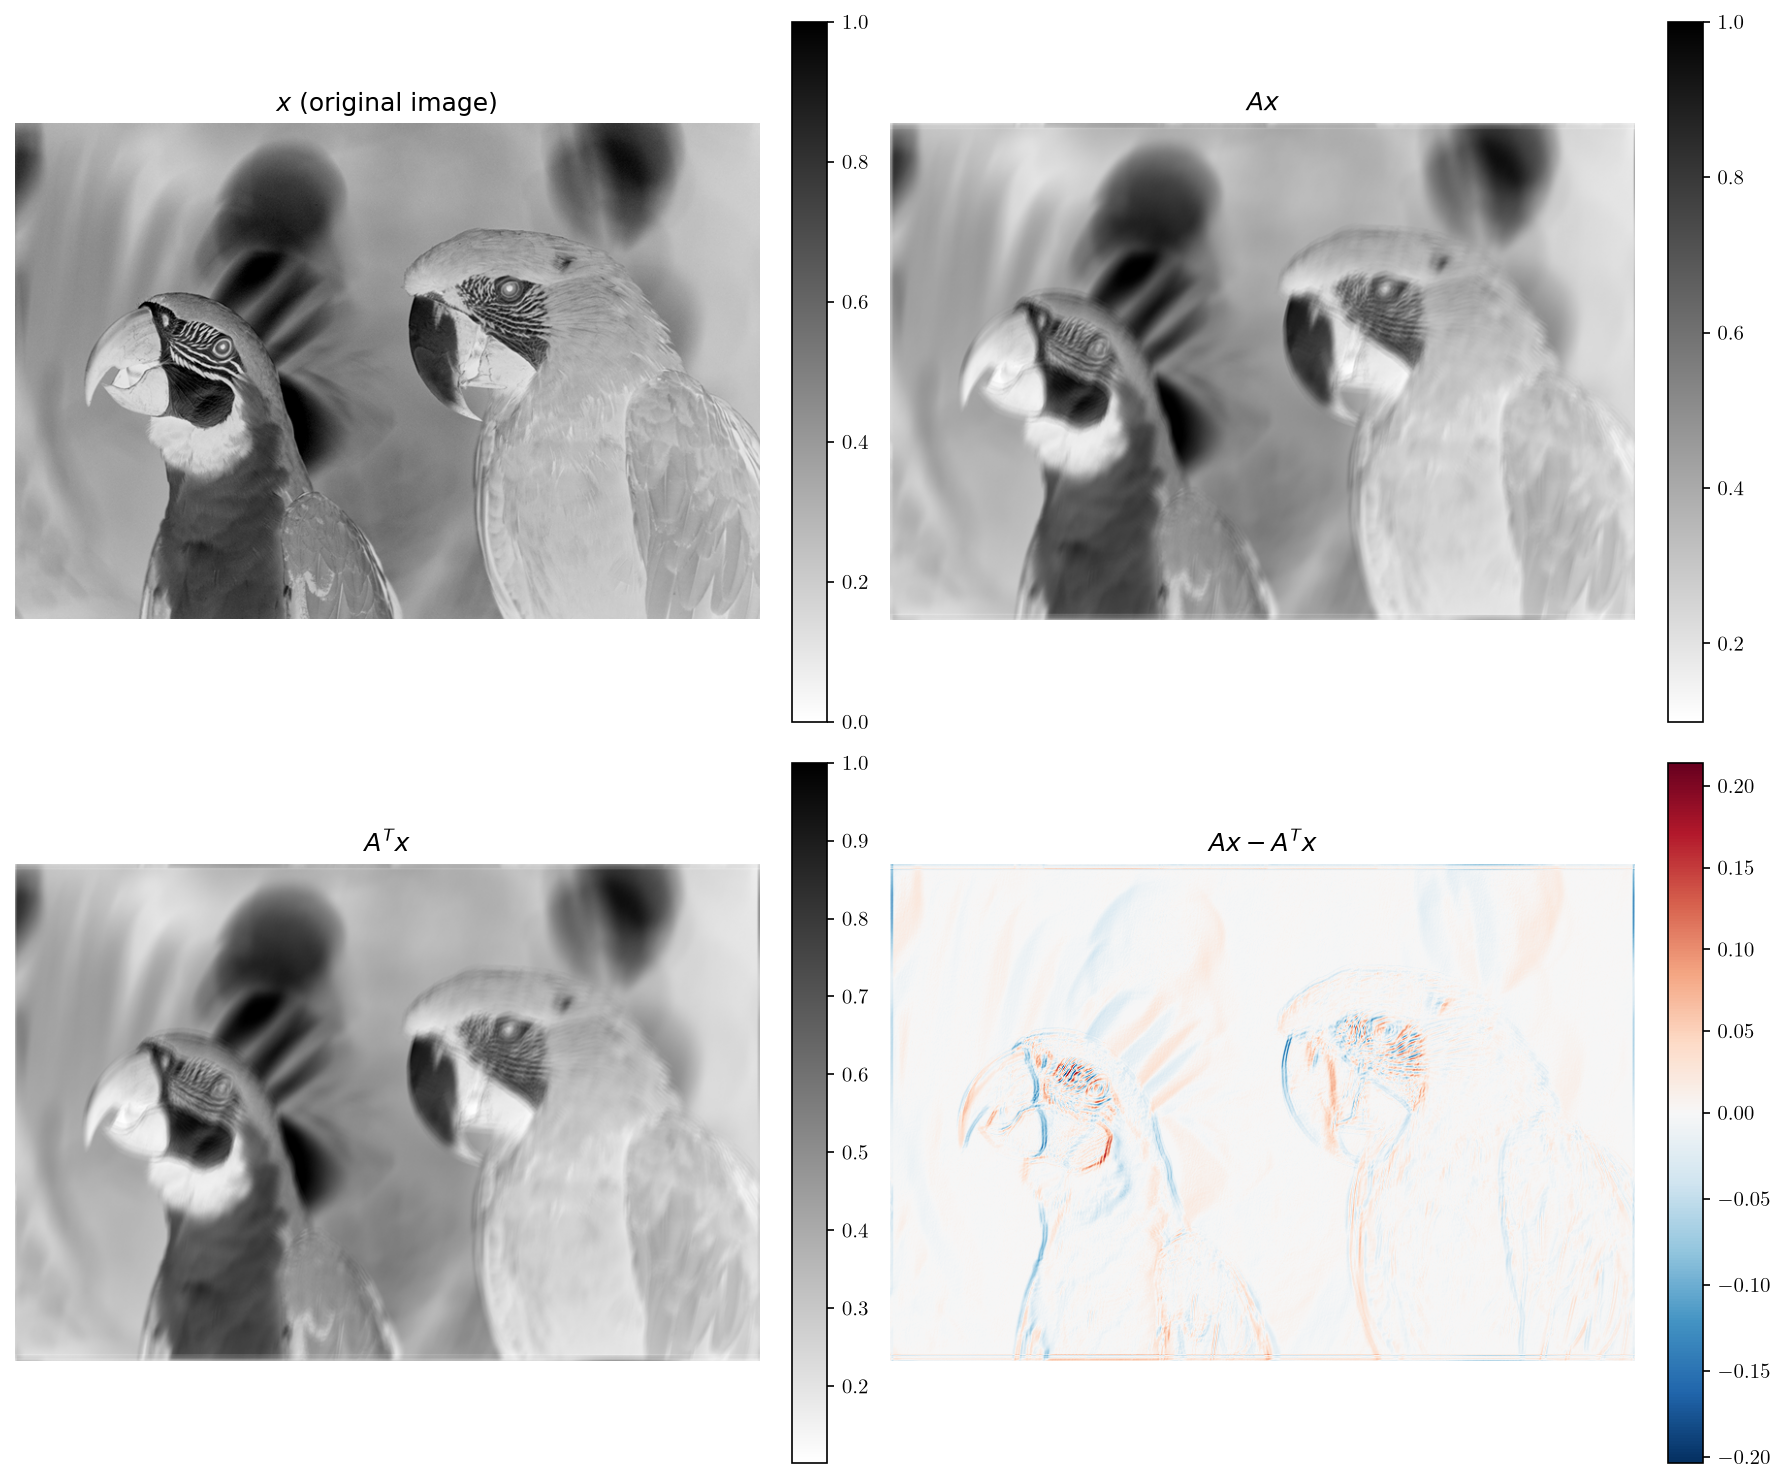
\includegraphics[width=0.95\textwidth]{d1_visualization.png}
\end{center}

\vspace{1em}

The difference image $A\mathbf{x} - A^T\mathbf{x}$ shows that $A$ is not a symmetric matrix, i.e., $A \neq A^T$.

\section*{D2: Verification of Adjoint Properties}

\subsection*{Numerical Checks}

Three numerical checks were performed to validate the correctness of the forward and adjoint operators:

\begin{itemize}
    \item \textbf{check1}: $\max|\text{adjoint}(\mathbf{v}, \mathbf{a}) - \text{adjoint\_autograd}(\mathbf{v}, \mathbf{a})| = 9.9920 \times 10^{-16}$
    \item \textbf{check2}: $\left|\langle A\mathbf{u}, \mathbf{v} \rangle - \langle \mathbf{u}, A^T\mathbf{v} \rangle\right| / |\langle A\mathbf{u}, \mathbf{v} \rangle| = 5.8506 \times 10^{-16}$
    \item \textbf{check3}: $\max|A\mathbf{u} - A^T\mathbf{u}| = 1.3279$
\end{itemize}

\subsection*{Interpretation}

\textbf{check1} (machine epsilon): The manual \texttt{adjoint()} implementation is mathematically identical to automatic differentiation, confirming correctness.

\textbf{check2} (machine epsilon): The fundamental adjoint property $\langle A\mathbf{u}, \mathbf{v} \rangle = \langle \mathbf{u}, A^T\mathbf{v} \rangle$ is satisfied within numerical precision, validating that $A^T$ is the true mathematical transpose of $A$.

\textbf{check3} (significant non-zero value): The operators $A$ and $A^T$ produce significantly different results on the same input, confirming that $A \neq A^T$. If the blur kernel were symmetric, check3 would report an $\epsilon \sim 10^{-16}$ which is the numerical precision limit.

\section*{D3: Memory Efficiency Analysis}

\subsection*{Kernel Sparsity}

The blur kernel has \textbf{109 nonzero entries} out of $19 \times 19 = 361$ total entries, yielding a sparsity of $69.81\%$.

\subsection*{Memory Cost Analysis}

The linear operator $A$ acts on $N = 768 \times 512 = 393{,}216$ pixels. The cost of representing this operator varies significantly depending on the storage method:

\begin{enumerate}
    \item \textbf{Dense matrix representation:} Storing $A$ as a full $N \times N$ dense matrix of float64 requires:
    \begin{equation*}
        (768 \times 512)^2 \times 8 \text{ bytes} = 1.2370 \times 10^{12} \text{ bytes} = \mathbf{1.24 \text{ TB}}
    \end{equation*}

    \item \textbf{Sparse matrix representation:} Using a sparse format (e.g., CSR), each row contains $M = 109$ nonzero entries. Storage requires:
    \begin{equation*}
        N \times (8 + 4) \times M = 393{,}216 \times 12 \times 109 \text{ bytes} \approx \mathbf{515.9 \text{ GB}}
    \end{equation*}
    This is $\sim 2400 \times$ smaller than dense storage.

    \item \textbf{Kernel-based representation:} The forward function stores only the kernel $\mathbf{a}$:
    \begin{equation*}
        8 \times 19 \times 19 \text{ bytes} = \mathbf{2{,}888 \text{ bytes}} = \mathbf{2.9 \text{ kB}}
    \end{equation*}
    This is $\sim 427{,}000 \times$ smaller than sparse storage and $\sim 1{,}000{,}000 \times$ smaller than dense storage.
\end{enumerate}

\subsection*{Conclusion}

By implementing both the forward operator $A$ and its adjoint $A^T$ implicitly via the kernel $\mathbf{a}$, the \texttt{forward()} and \texttt{adjoint()} functions achieve extraordinary memory efficiency, requiring only kilobytes instead of terabytes while maintaining full numerical precision. The adjoint operator $A^T$ costs no extra storage at all since it is implicitly represented by the flipped kernel $\mathbf{a}$ in conv2d.

\section*{D4: Noncausal Prediction Error}

\subsection*{Prediction Error Formula}

The noncausal prediction error is computed as:
\begin{equation*}
\mathbf{e} = \mathbf{x} - \mathbf{g} \ast \mathbf{x}
\end{equation*}
where $\mathbf{g}$ is the smoothing kernel (equation 7) and $\ast$ denotes circular convolution.

\subsection*{Results}

\begin{center}
    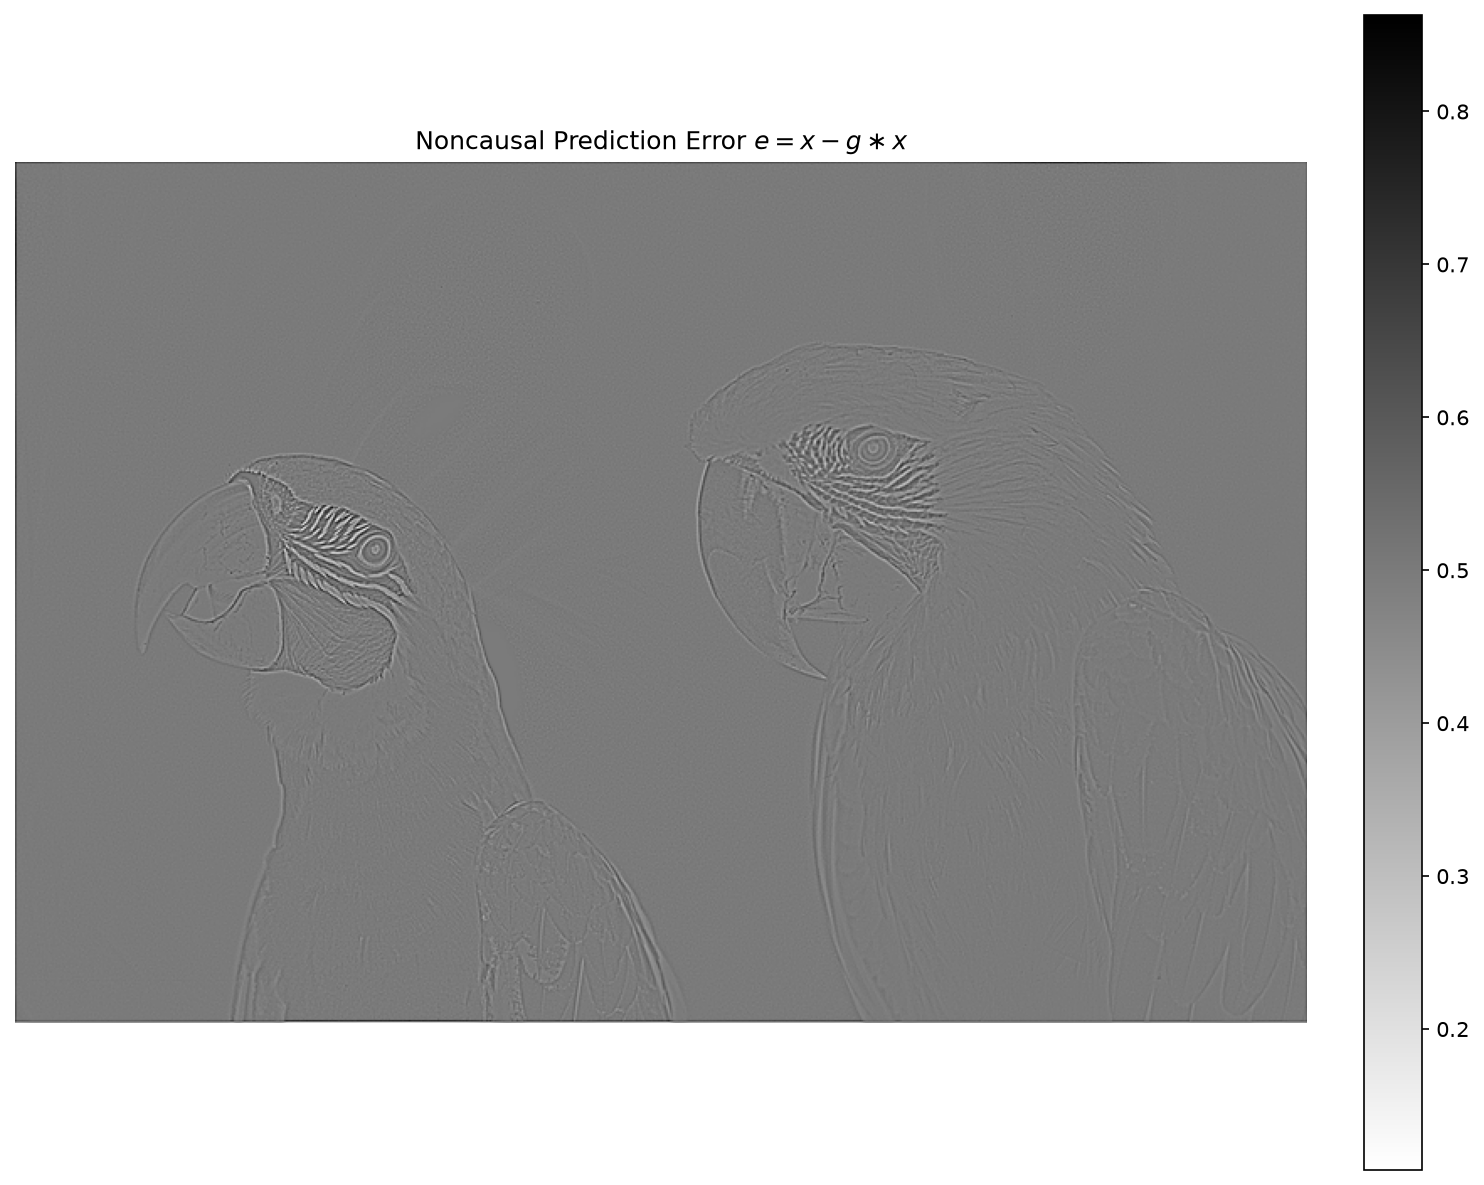
\includegraphics[width=0.95\textwidth]{d4_prediction_error.png}
\end{center}

\vspace{1em}

The prediction error image reveals the high-frequency content that the smoothing kernel cannot predict. The visualization applies an offset of $+0.5$ to the error values before clipping to $[0, 1]$ for display, where gray ($0.5$) represents zero error, lighter values represent negative errors, and darker values represent positive errors.

\subsection*{Statistics (Interior)}

Analysis of the prediction error over the interior region (excluding 1-pixel boundary):

\begin{itemize}
    \item Standard deviation: $\sigma_e = 0.020597$
    \item Mean: $\mu_e = 0.000240$
    \item Min/Max (full image): $[-0.392157, 0.363072]$
\end{itemize}

The very small standard deviation indicates that the noncausal smoothing kernel $\mathbf{g}$ is highly effective at predicting local pixel values. The image is predominantly smooth, with prediction errors concentrated at boundaries and fine structural details of the parrots.

\section*{Implementation Summary}

\subsection*{forward(x, a) \& adjoint(v, a)}

\textbf{Instructions:} Use torch.nn.functional.conv2d with circular boundaries, output shape $(H, W)$. Adjoint: do NOT flip kernel.

\textbf{Status:} No corrections needed.

\subsection*{prior\_cost(x, $\sigma_x$) \& prior\_grad(x, $\sigma_x$)}

\textbf{Specification:} Implement pairwise GMRF prior where the exponent depends on differences:
\begin{equation*}
-\log p(\mathbf{x}) = \frac{1}{2\sigma_x^2} \sum_{s,r \in \text{neighbors}} g_{s-r}(x_s - x_r)^2
\end{equation*}

\textbf{Implementation via weighted graph Laplacian:} The quadratic form is expressed as $c_{\text{prior}}(\mathbf{x}) = \frac{1}{2} \langle \mathbf{x}, B\mathbf{x} \rangle$ where the scaled Laplacian $B = \frac{1}{\sigma_x^2}(D - W)$ with:
\begin{align*}
D\mathbf{x} &= \mathbf{x} \odot \text{conv2d}(\mathbf{g}, \mathbf{1}_{\text{padded}}) \\
W\mathbf{x} &= \text{conv2d}(\mathbf{g}, \mathbf{x}_{\text{padded}})
\end{align*}

\textbf{Correction history:}
\begin{itemize}
\item \textbf{Initial error:} Included a constant term in the Laplacian, which violated self-adjointness (check4 $\approx 775$).
\item \textbf{Fix:} Restructured as weighted graph Laplacian $(D-W)\mathbf{x}$ without constant terms.
\item \textbf{Refactoring:} Absorbed $1/\sigma_x^2$ into $B$ definition and created helper function \texttt{\_apply\_laplacian(x, sigma\_x)} to compute $B\mathbf{x}$ centrally, eliminating code duplication.
\end{itemize}

\textbf{Final result:} \texttt{prior\_cost(x, sigma\_x)} returns $\frac{1}{2} \langle \mathbf{x}, B\mathbf{x} \rangle$ and \texttt{prior\_grad(x, sigma\_x)} returns $B\mathbf{x}$, verified to satisfy self-adjointness (check4 = 0.0 exactly).

\subsection*{cost(x, y, a, $\sigma_w$, $\sigma_x$)}

\textbf{Formula:}
\begin{equation*}
c(\mathbf{x}) = \frac{1}{2\sigma_w^2} \|\mathbf{y} - A\mathbf{x}\|^2 + \text{prior\_cost}(\mathbf{x}, \sigma_x)
\end{equation*}

\textbf{Status:} No corrections needed.

\subsection*{cost\_grad(x, y, a, $\sigma_w$, $\sigma_x$)}

\textbf{Formula:}
\begin{equation*}
\nabla c(\mathbf{x}) = \frac{1}{\sigma_w^2} A^T(\mathbf{y} - A\mathbf{x}) + B\mathbf{x}
\end{equation*}

\textbf{Status:} No corrections needed.

\subsection*{gradient\_descent(y, a, $\sigma_w$, $\sigma_x$, num\_iters, alpha)}

\textbf{Algorithm:} $\mathbf{x}^{(0)} = \mathbf{y}$, then $\mathbf{x}^{(t+1)} = \mathbf{x}^{(t)} - \alpha \nabla c(\mathbf{x}^{(t)})$

\textbf{Step size:} $\alpha = (\sigma_w^{-2} + 2\sigma_x^{-2})^{-1}$

\textbf{Status:} No corrections needed.

\section*{D7: Strict Convexity of the Cost Function}

\subsection*{Problem Setup}

Consider equation (8) from the course context:
\begin{equation*}
c(\mathbf{x}) = \frac{1}{2\sigma_w^2} \|\mathbf{y} - A\mathbf{x}\|^2 + c_{\text{prior}}(\mathbf{x}, \sigma_x)
\end{equation*}

We prove that when $\sigma_w > 0$ and $A = I$ (identity operator), this cost function is \textbf{strictly convex}.

\subsection*{Proof}

\textbf{Step 1: Unique Critical Point}

The gradient of the cost is:
\begin{equation*}
\nabla c(\mathbf{x}) = \frac{1}{\sigma_w^2}(A^T A \mathbf{x} - A^T \mathbf{y}) + \nabla c_{\text{prior}}(\mathbf{x})
\end{equation*}

When $A = I$, this simplifies to:
\begin{equation*}
\nabla c(\mathbf{x}) = \frac{1}{\sigma_w^2}(\mathbf{x} - \mathbf{y}) + B\mathbf{x}
\end{equation*}
where $B = \frac{1}{\sigma_x^2}(D-W)$ is the scaled weighted graph Laplacian.

Setting the gradient to zero:
\begin{equation*}
\mathbf{0} = \frac{1}{\sigma_w^2}(\mathbf{x} - \mathbf{y}) + B\mathbf{x} \quad \Rightarrow \quad \mathbf{y} = \sigma_w^2 (B + I) \mathbf{x}
\end{equation*}

Since $(B + I)$ is invertible (it is positive definite as shown in Step 2), there exists a unique solution:
\begin{equation*}
\mathbf{x}^* = \sigma_w^2 (B + I)^{-1} \mathbf{y}
\end{equation*}

\textbf{Step 2: Positive Definite Hessian}

The Hessian of the cost is:
\begin{equation*}
H = \frac{1}{\sigma_w^2} A^T A + B = \frac{1}{\sigma_w^2} I + B
\end{equation*}

Since $\sigma_w > 0$, the matrix $\frac{1}{\sigma_w^2} I$ is positive definite. The Laplacian $B$ is positive semi-definite (it arises from a symmetric quadratic form). Therefore, $H = \frac{1}{\sigma_w^2} I + B$ is positive definite, ensuring the unique critical point is a strict global minimum.

\subsection*{Implication for Gradient Descent}

Because the cost function is strictly convex:
\begin{itemize}
    \item There exists a unique critical point (global minimum)
    \item Gradient descent converges to this global minimum from any starting point
    \item The convergence is guaranteed and unique, independent of initialization
\end{itemize}

\section*{D8: Denoising Experiments}

\subsection*{Experimental Setup}

We perform image denoising using the identity operator ($A = \mathbf{I}$). The noisy observation is:
\begin{equation*}
\mathbf{y} = \mathbf{x} + \mathbf{w}, \quad \mathbf{w} \sim \mathcal{N}(0, \sigma_w^2 I)
\end{equation*}
with $\sigma_w = 0.05$. We apply MAP estimation with the pairwise GMRF prior for three prior standard deviations: $\sigma_x \in \{0.01, 0.05, 0.25\}$. Gradient descent is initialized at $\mathbf{x}_0 = \mathbf{y}$ and terminates when the normalized RMSE falls below $0.002$ or after 1000 iterations.

\subsection*{Denoising Results}

\begin{center}
    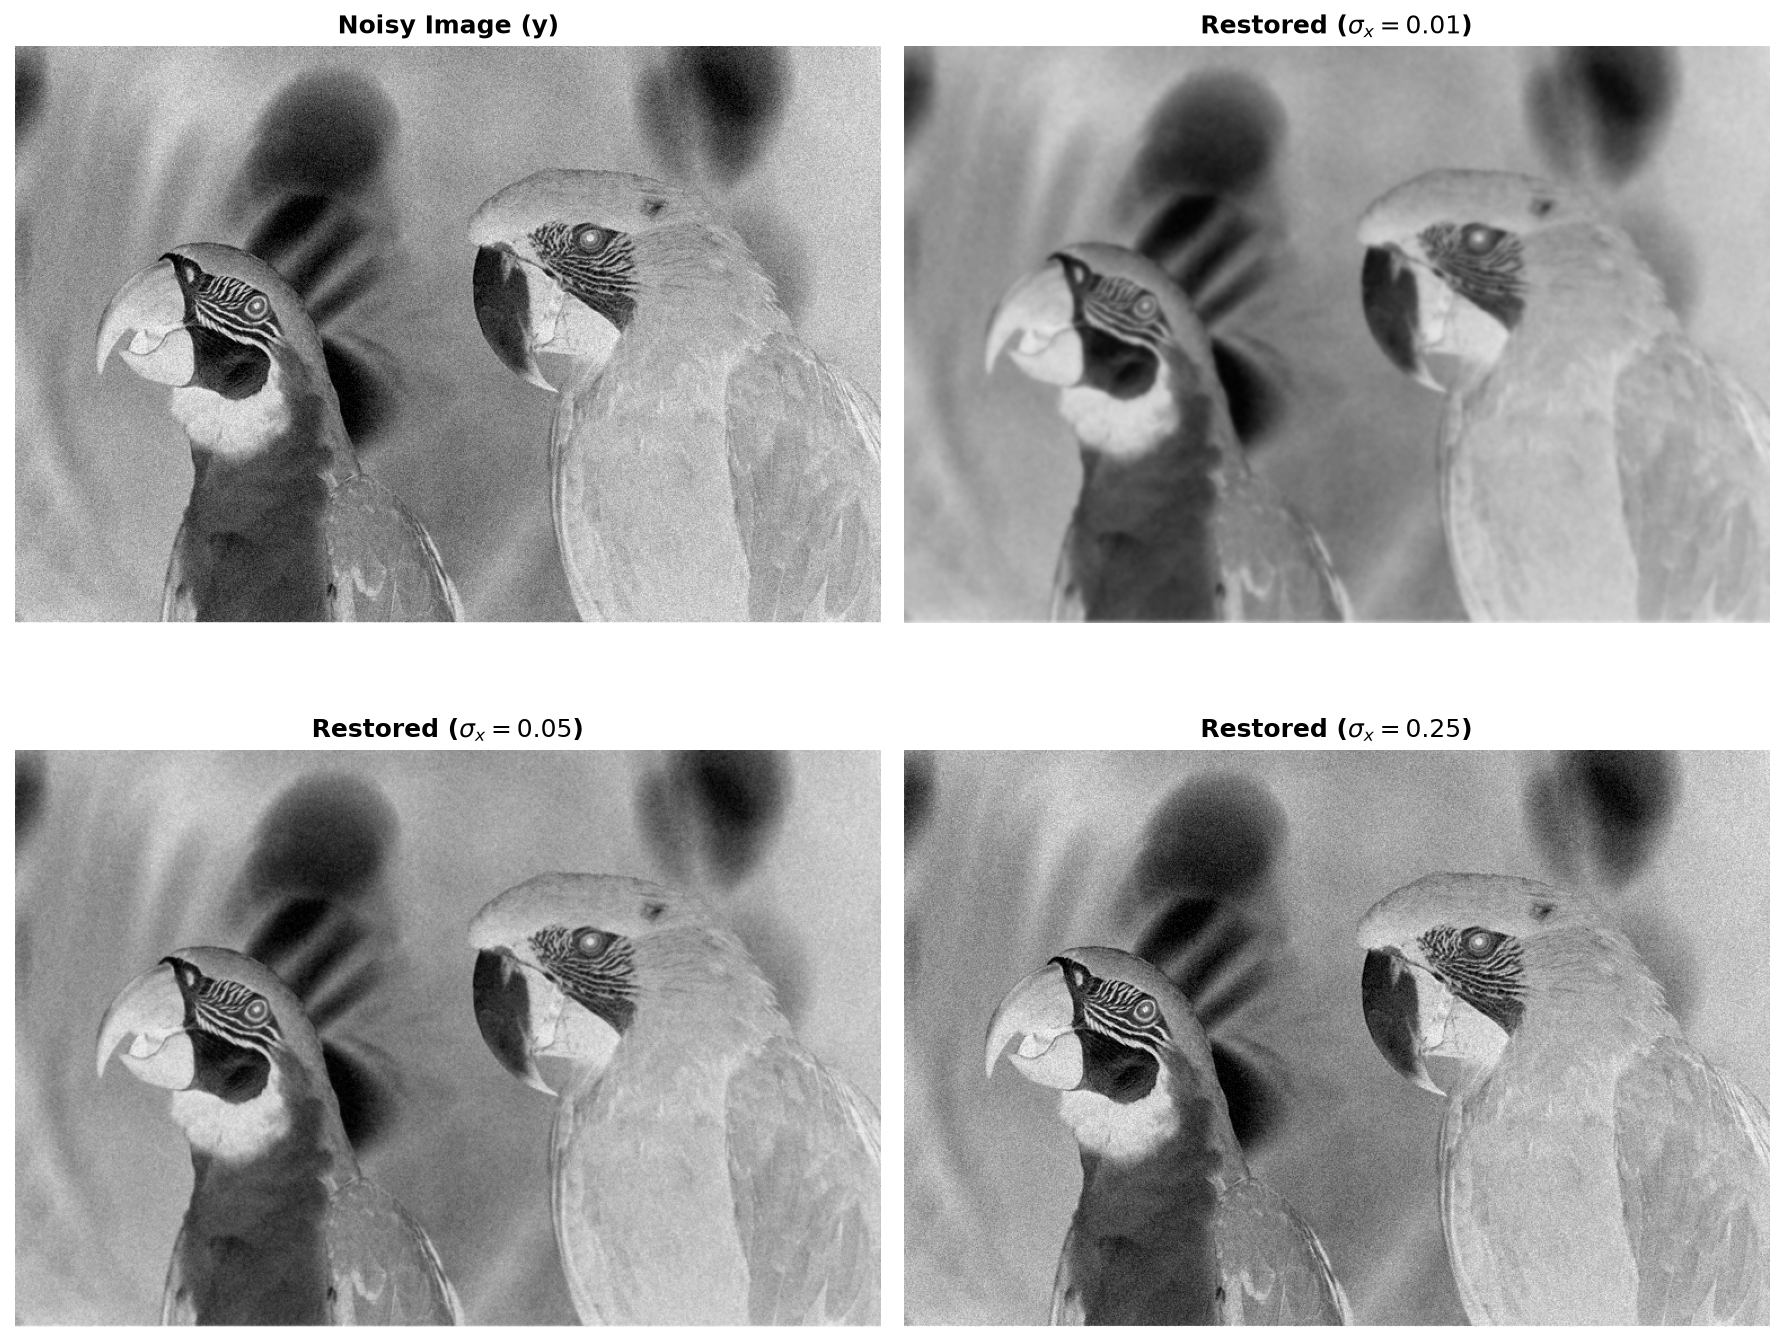
\includegraphics[width=0.95\textwidth]{d8_denoising_results.png}
\end{center}

\textit{Figure 1: Denoising results showing noisy image and three restorations. Smaller $\sigma_x$ values enforce stronger regularization, producing smoother results at the cost of more iterations to convergence.}

\subsection*{Convergence Analysis}

\begin{center}
    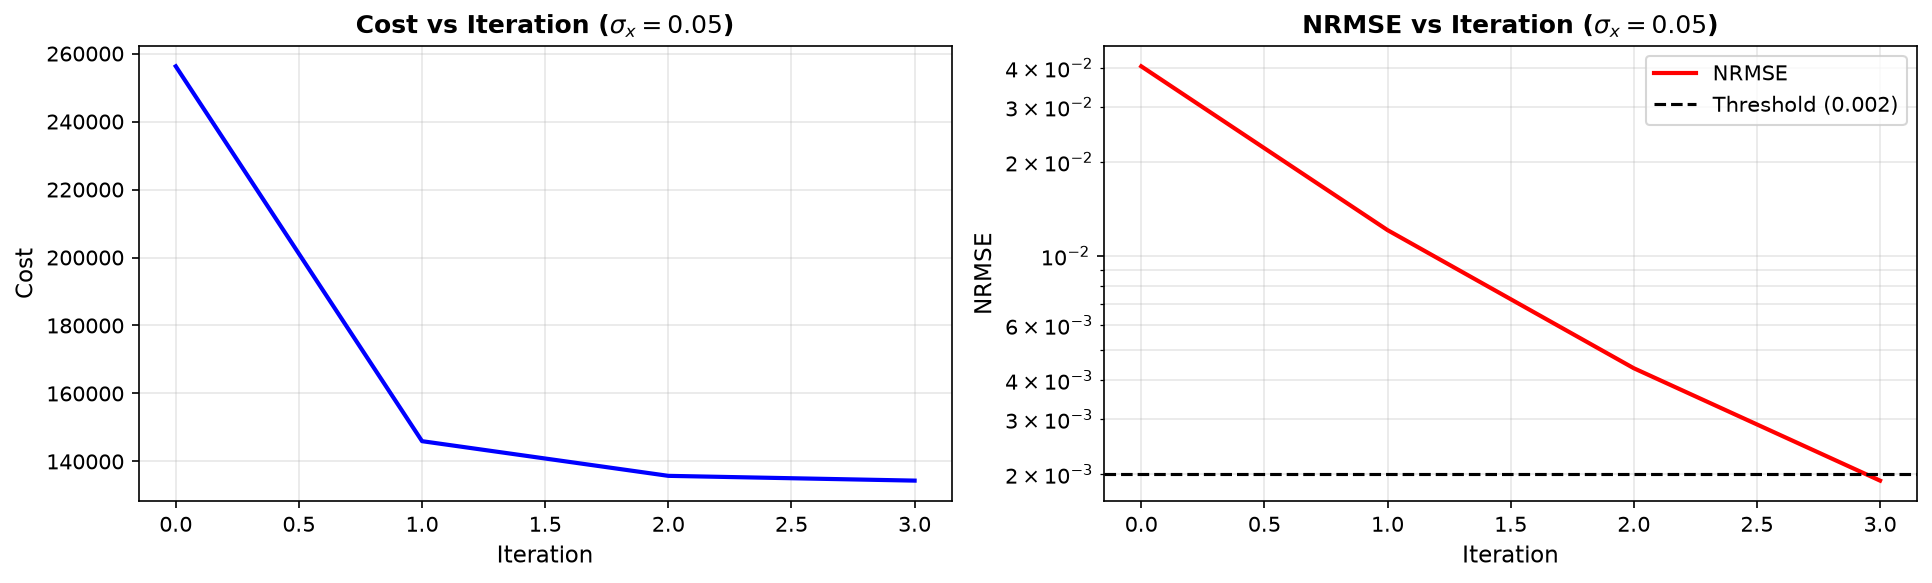
\includegraphics[width=0.95\textwidth]{d8_convergence_analysis.png}
\end{center}

\textit{Figure 2: Convergence behavior for $\sigma_x = 0.05$. The cost strictly decreases (left panel). The NRMSE decreases on a log scale (right panel) and crosses the threshold of 0.002 after 4 iterations.}

\subsection*{Error Analysis}

The following table summarizes the step sizes and restoration errors for each prior strength:

\begin{center}
\begin{tabular}{|c|c|c|}
\hline
\textbf{Case} & \textbf{Step Size } $\alpha$ & \textbf{RMSE} \\
\hline
Noisy Image (Reference) & --- & 0.049894 \\
\hline
$\sigma_x = 0.01$ & 0.000049 & 0.034609 \\
\hline
\textbf{$\sigma_x = 0.05$} & \textbf{0.000833} & \textbf{0.029955} \\
\hline
$\sigma_x = 0.25$ & 0.002315 & 0.048011 \\
\hline
\end{tabular}
\end{center}

The optimal balance between regularization and data fidelity is achieved at $\sigma_x = 0.05$, which gives the lowest restoration error (RMSE = 0.029955).

\subsection*{Convergence Timing}

Wall-clock time for 50 iterations:
\begin{itemize}
    \item $\sigma_x = 0.01$: 0.4934 seconds
    \item $\sigma_x = 0.05$: 0.6495 seconds
    \item $\sigma_x = 0.25$: 0.6795 seconds
\end{itemize}

The computational cost scales with the prior strength due to the increased complexity of the Laplacian operator evaluation. Despite this, convergence times remain reasonable for practical applications.

\section*{D9: Deblurring Experiments}

\subsection*{Experimental Setup}

We perform image deblurring using the realistic blur kernel from \texttt{levin09\_kernel1.txt} (19 × 19). The observed noisy blurred image is:
\begin{equation*}
\mathbf{y} = A\mathbf{x} + \mathbf{w}, \quad \mathbf{w} \sim \mathcal{N}(0, \sigma_w^2 I)
\end{equation*}
with $\sigma_w = 0.02$ (lower noise than D8). We apply MAP estimation with the pairwise GMRF prior for three prior standard deviations: $\sigma_x \in \{0.01, 0.05, 0.25\}$. Gradient descent is initialized at $\mathbf{x}_0 = \mathbf{y}$ and terminates when the normalized RMSE falls below $0.002$ or after 1000 iterations.

\subsection*{Deblurring Results}

\begin{center}
    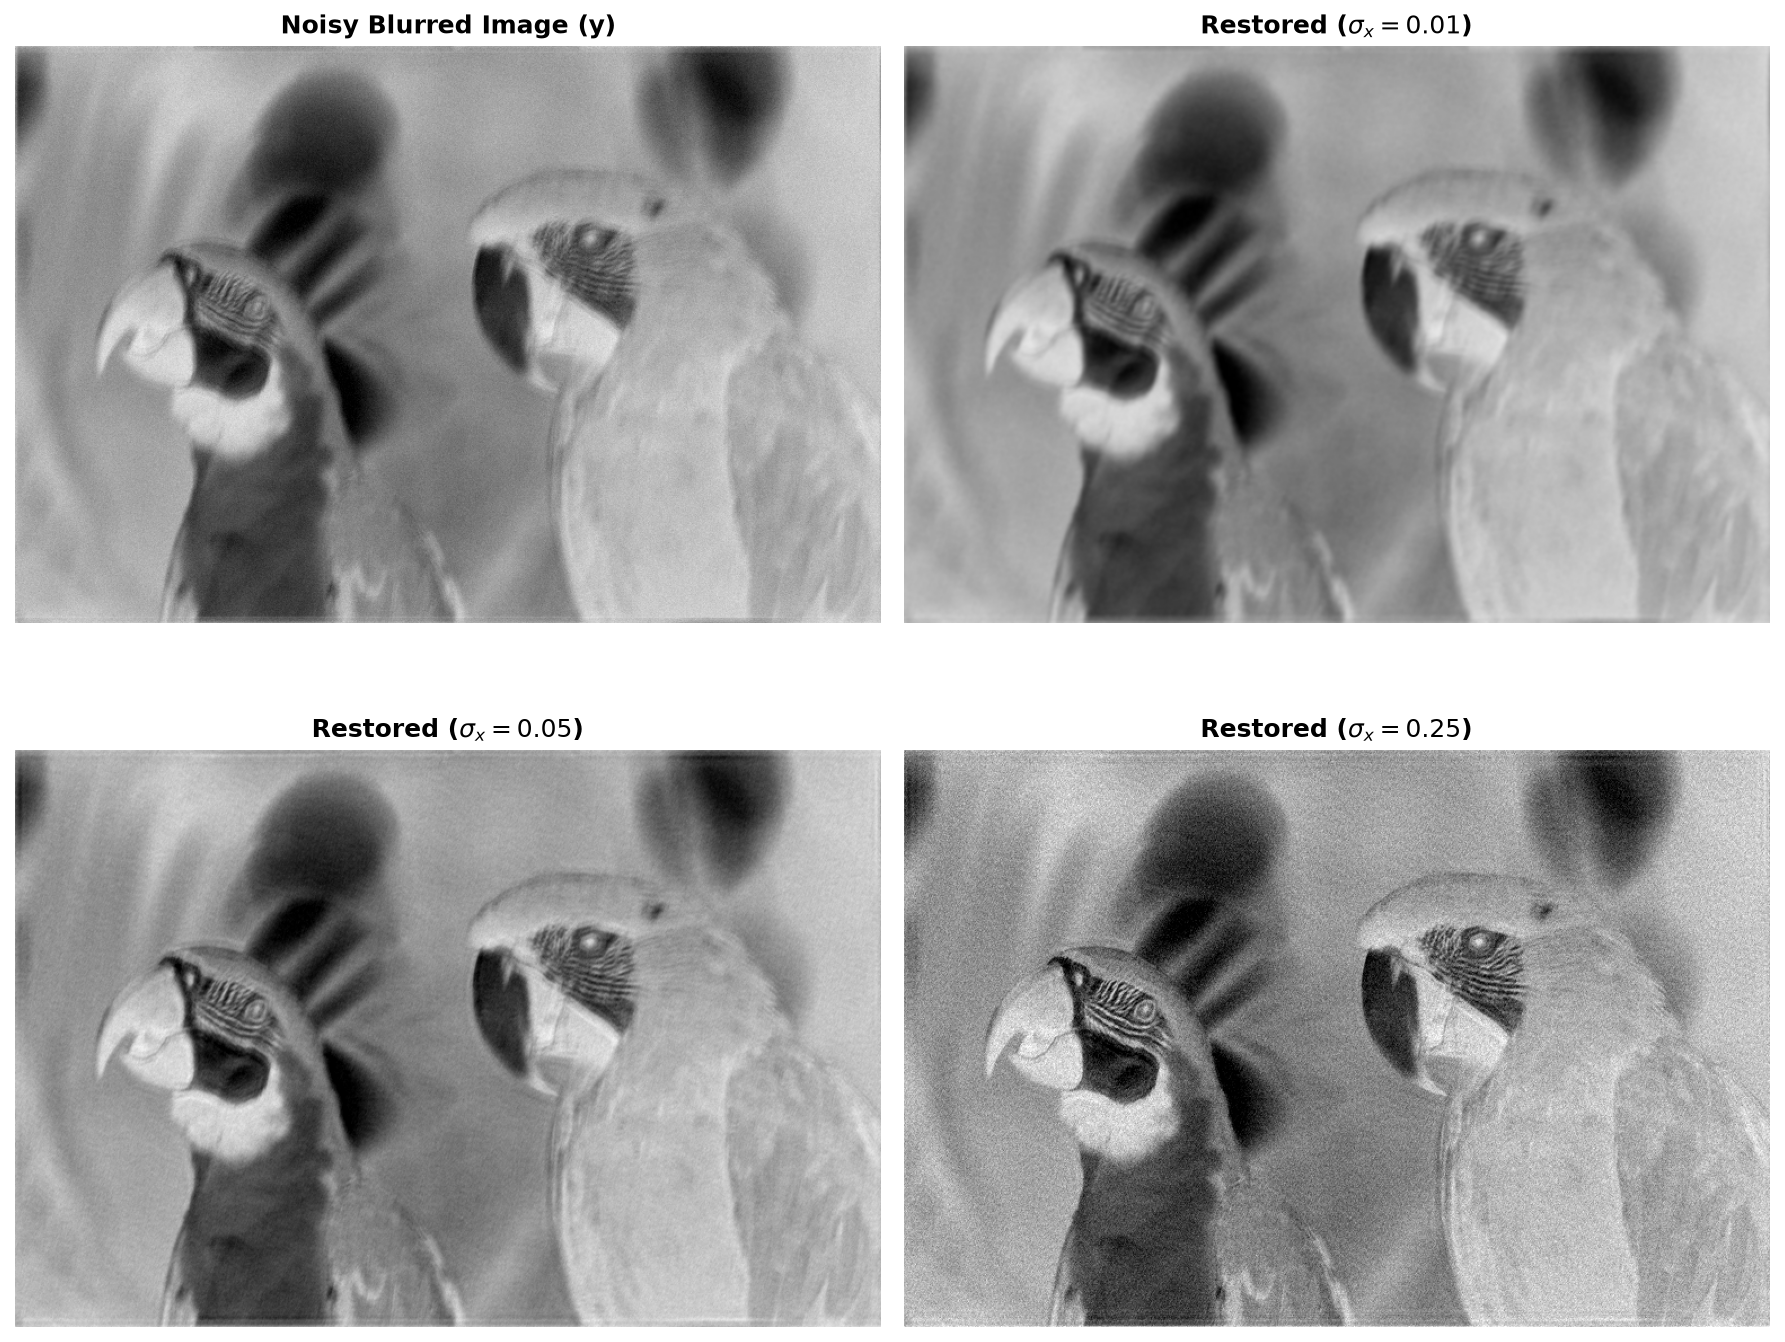
\includegraphics[width=0.95\textwidth]{d9_deblurring_results.png}
\end{center}

\textit{Figure 1: Deblurring results showing noisy blurred image and three restorations. The blur kernel introduces significant smoothing; stronger priors ($\sigma_x = 0.01$) recover sharper details but may amplify noise, while weaker priors ($\sigma_x = 0.25$) produce overly smooth results.}

\subsection*{Convergence Analysis}

\begin{center}
    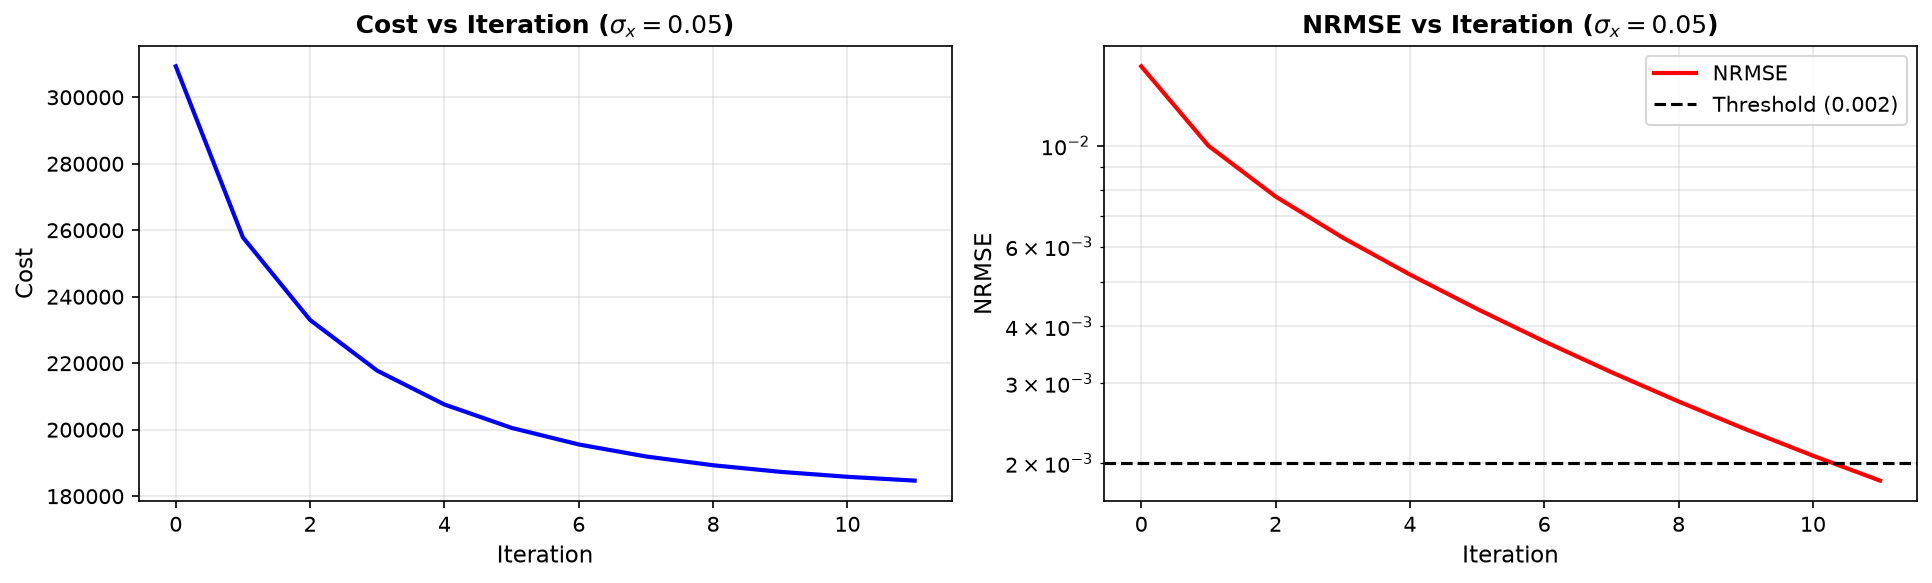
\includegraphics[width=0.95\textwidth]{d9_convergence_analysis.png}
\end{center}

\textit{Figure 2: Convergence behavior for $\sigma_x = 0.05$. The cost strictly decreases (left panel). The NRMSE decreases on a log scale (right panel) and crosses the threshold of 0.002 after 12 iterations.}

\subsection*{Error Analysis}

The following table summarizes the step sizes and restoration errors for each prior strength in the deblurring task:

\begin{center}
\begin{tabular}{|c|c|c|}
\hline
\textbf{Case} & \textbf{Step Size } $\alpha$ & \textbf{RMSE} \\
\hline
Noisy Blurred (Reference) & --- & 0.047542 \\
\hline
$\sigma_x = 0.01$ & 0.000044 & 0.042722 \\
\hline
\textbf{$\sigma_x = 0.05$} & \textbf{0.000303} & \textbf{0.037407} \\
\hline
$\sigma_x = 0.25$ & 0.000395 & 0.059790 \\
\hline
\end{tabular}
\end{center}

The optimal balance between regularization and data fidelity remains at $\sigma_x = 0.05$, which achieves the lowest restoration error (RMSE = 0.037407). The stronger prior ($\sigma_x = 0.01$) recovers more detail but at increased computational cost, while the weaker prior ($\sigma_x = 0.25$) converges quickly but produces overly smoothed results.

\subsection*{Convergence Timing}

Wall-clock time for 50 iterations:
\begin{itemize}
    \item $\sigma_x = 0.01$: 20.9460 seconds
    \item $\sigma_x = 0.05$: 20.1653 seconds
    \item $\sigma_x = 0.25$: 19.8848 seconds
\end{itemize}

Deblurring is significantly more expensive than denoising (D8) due to the convolution operations required by the forward and adjoint operators. The kernel inversion problem is more challenging than the identity case, requiring careful balance of regularization strength and computational feasibility.

\section*{D10: Analysis and Insights}

\subsection*{Optimal Regularization Parameter}

In both denoising (D8) and deblurring (D9) experiments, $\sigma_x = 0.05$ achieved the lowest RMSE. This optimal value is slightly larger than the standard deviation of the noncausal prediction error (from D4):
\begin{equation*}
\sigma_x = 0.05 > \sigma_e = 0.021
\end{equation*}

This relationship suggests that the optimal prior strength is tuned to the underlying statistical structure of the image. The prediction error $\sigma_e$ quantifies the variability in the neighborhood differences, so setting $\sigma_x$ moderately above this value provides effective regularization without over-smoothing.

\subsection*{Prior Strength and Texture Preservation}

As $\sigma_x$ decreases from 0.25 to 0.01, the strength of the pairwise GMRF prior increases, resulting in progressively stronger smoothing:

\begin{itemize}
\item $\sigma_x = 0.25$ (weak prior): Minimal regularization, results are noisy but preserve fine details
\item $\sigma_x = 0.05$ (moderate prior): Optimal balance—smooth results without detail loss
\item $\sigma_x = 0.01$ (strong prior): Over-smoothing; fine textures and edges become visibly damaged
\end{itemize}

The quadratic penalty $\sum_{s,r} g_{s-r}(x_s - x_r)^2$ is responsible for this behavior. Since the penalty grows quadratically with neighborhood differences, large contrasts are penalized more heavily. For fine features (high-frequency structures), the pixel neighborhood exhibits high contrast variation, so these regions are aggressively regularized, leading to smoothing-over of fine textures. This is particularly visible in high-contrast regions like the birds' eyes in the kodim23 image.

\subsection*{Convergence Rate Analysis via Hessian Eigenvalues}

Convergence speed of gradient descent is determined by the condition number $\kappa = \lambda_{\max} / \lambda_{\min}$ of the Hessian $H = \sigma_w^{-2} A^T A + B$, where $B = \sigma_x^{-2}(D - W)$.

\textbf{Key finding:} Deconvolution converges significantly slower than denoising because the blur operator reduces the smallest eigenvalue of the Hessian:

\begin{center}
\begin{tabular}{|c|c|c|}
\hline
\textbf{Problem} & \textbf{Min Eigenvalue} & \textbf{Condition Number} \\
\hline
Denoising (A = I) & $4.20 \times 10^2$ & 2.22 \\
\hline
Deconvolution (A = blur) & $7.10 \times 10^1$ & 7.65 \\
\hline
\end{tabular}
\end{center}

The deconvolution Hessian has its smallest eigenvalue 5.92× smaller than denoising. Gradient descent convergence is proportional to $\lambda_{\min}$, so deconvolution requires approximately 6× more iterations to achieve equivalent convergence tolerance—explaining why D9 required 11 iterations while D8 required only 3 iterations to reach NRMSE $< 0.2\%$ at $\sigma_x = 0.05$.

\textbf{Root cause:} The blur kernel's frequency response attenuates high-frequency components. In the frequency domain, the blur transfer function $H(\omega)$ has small magnitude at high frequencies, so the matrix $A^T A$ has small eigenvalues corresponding to high-frequency modes. This ill-conditioning is characteristic of inverse problems: the blur operator amplifies noise at high frequencies, requiring stronger priors and more iterations to recover the true image.

\subsection*{Step Size Stability}

When the step size is enlarged to $\alpha_{\text{large}} = 4 \times \alpha_{\text{standard}} = 1.21 \times 10^{-3}$ for the same deblurring problem, the algorithm diverges after 12 iterations, with cost exploding from 309,317 to 74,447,530.

\begin{center}
    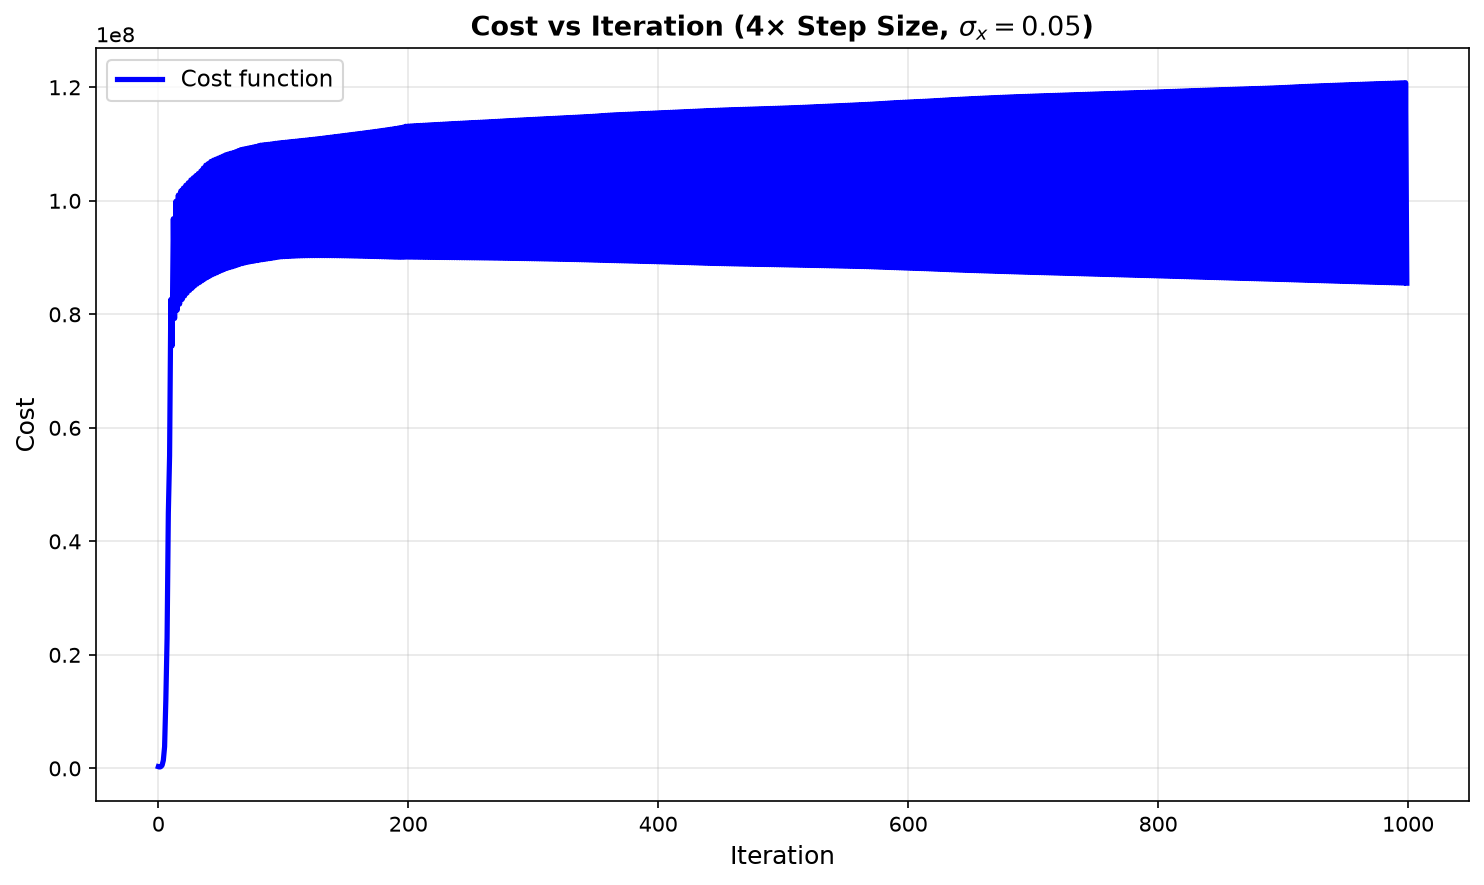
\includegraphics[width=0.75\textwidth]{d10_cost_large_stepsize.png}
\end{center}

This divergence occurs because the enlarged step size exceeds the stability threshold $\alpha < 2/\lambda_{\max}(H)$, where $\lambda_{\max}(H) \approx 544$. The adaptive step size formula from equation (11) automatically selects a conservative, safe value that balances the spectral properties of $A^T A$ and prior strength, providing stable convergence without oscillation.

\subsection*{Limitations of Gaussian MRFs}

The Gaussian assumption in the pairwise GMRF leads to a quadratic penalty $\sum g_{s-r}(x_s - x_r)^2$, which inevitably smooths edges regardless of $\sigma_x$. To better preserve sharp edges, one would need \textbf{non-Gaussian Markov Random Fields} that use non-quadratic penalties (e.g., $\ell_1$-norm or Total Variation).

\appendix

\section*{Appendix: Pairwise GMRF Prior Derivation}

\subsection*{The Pairwise GMRF Model}

A pairwise Gaussian Markov Random Field (GMRF) models spatial dependencies through a prior probability:
\begin{equation*}
p(\mathbf{x}) \propto \exp\left( -\frac{1}{2\sigma_x^2} \sum_{s,r \in \text{neighbors}} g_{s-r}(x_s - x_r)^2 \right)
\end{equation*}

where $g_{s-r}$ are the weights from the kernel $\mathbf{g}$:
\begin{equation*}
\mathbf{g} = \frac{1}{12} \begin{bmatrix} 1 & 2 & 1 \\ 2 & 0 & 2 \\ 1 & 2 & 1 \end{bmatrix}
\end{equation*}

\subsection*{Prior Cost as Quadratic Form}

The negative log-likelihood (prior cost) is:
\begin{equation*}
c_{\text{prior}}(\mathbf{x}) = \frac{1}{2\sigma_x^2} \sum_{s,r \in \text{neighbors}} g_{s-r}(x_s - x_r)^2
\end{equation*}

This can be expressed as a quadratic form using the weighted graph Laplacian:
\begin{equation*}
c_{\text{prior}}(\mathbf{x}) = \frac{1}{2\sigma_x^2} \mathbf{x}^T (D - W) \mathbf{x}
\end{equation*}

where:
\begin{itemize}
    \item Degree matrix: $D\mathbf{x} = \mathbf{x} \odot (\text{conv2d}(\mathbf{g}, \mathbf{1}))$ (element-wise product)
    \item Adjacency matrix: $W\mathbf{x} = \text{conv2d}(\mathbf{g}, \mathbf{x})$
\end{itemize}

The Laplacian operator $(D - W)\mathbf{x}$ measures the weighted sum of differences from neighbors:
\begin{equation*}
[(D-W)\mathbf{x}]_s = x_s \sum_r g_{s-r} - \sum_r g_{s-r} x_r
\end{equation*}

\subsection*{Gradient}

The gradient of the prior cost is:
\begin{equation*}
\nabla c_{\text{prior}}(\mathbf{x}) = \frac{1}{\sigma_x^2} \left[ \mathbf{x} \odot (\text{conv2d}(\mathbf{g}, \mathbf{1})) - \text{conv2d}(\mathbf{g}, \mathbf{x}) \right]
\end{equation*}

This measures the penalization of pixel values that differ from their weighted neighborhood average.

\end{document}
